\documentclass[12pt]{report}
\usepackage[spanish]{babel}
\usepackage[utf8]{inputenc}
\usepackage{amsmath}
\usepackage{amssymb}
\usepackage{amsthm}
\usepackage{graphics}
\usepackage{subfigure}
\usepackage{lipsum}
\usepackage{array}
\usepackage{multicol}
\usepackage{enumerate}
\usepackage[framemethod=TikZ]{mdframed}
\usepackage[a4paper, margin = 1.5cm]{geometry}
\usepackage{tikz}
\usepackage{pgffor}
\usepackage{ifthen}
\usepackage{listings}
\usepackage{hyperref}
\usepackage{xcolor}

%Gestión de Hipervínculos

\hypersetup{
    colorlinks=true,
    linkcolor=black,
    filecolor=magenta,      
    urlcolor=cyan
}

%Gestión de Código de Programación

\definecolor{listing-background}{HTML}{F7F7F7}
\definecolor{listing-rule}{HTML}{B3B2B3}
\definecolor{listing-numbers}{HTML}{B3B2B3}
\definecolor{listing-text-color}{HTML}{000000}
\definecolor{listing-keyword}{HTML}{435489}
\definecolor{listing-keyword-2}{HTML}{1284CA} % additional keywords
\definecolor{listing-keyword-3}{HTML}{9137CB} % additional keywords
\definecolor{listing-identifier}{HTML}{435489}
\definecolor{listing-string}{HTML}{00999A}
\definecolor{listing-comment}{HTML}{8E8E8E}

\lstdefinestyle{myStyle}{
    language         = java,
    alsolanguage     = scala,
    numbers          = left,
    xleftmargin      = 2.7em,
    framexleftmargin = 2.5em,
    backgroundcolor  = \color{gray!15},
    basicstyle       = \color{listing-text-color}\linespread{1.0}\ttfamily,
    breaklines       = true,
    frameshape       = {RYR}{Y}{Y}{RYR},
    rulecolor        = \color{black},
    tabsize          = 2,
    numberstyle      = \color{listing-numbers}\linespread{1.0}\small\ttfamily,
    aboveskip        = 1.0em,
    belowskip        = 0.1em,
    abovecaptionskip = 0em,
    belowcaptionskip = 1.0em,
    keywordstyle     = {\color{listing-keyword}\bfseries},
    keywordstyle     = {[2]\color{listing-keyword-2}\bfseries},
    keywordstyle     = {[3]\color{listing-keyword-3}\bfseries\itshape},
    sensitive        = true,
    identifierstyle  = \color{listing-identifier},
    commentstyle     = \color{listing-comment},
    stringstyle      = \color{listing-string},
    showstringspaces = false,
}

\lstset{style = myStyle}

%Gestión de Marca de Agua

\newcounter{it}
\newcommand*\watermarktext[1]{\begin{tabular}{c}
    \setcounter{it}{1}%
    \whiledo{\theit<100}{%
    \foreach \col in {0,...,15}{#1\ \ } \\ \\ \\
    \stepcounter{it}%
    }
    \end{tabular}
    }

\AddToHook{shipout/foreground}{
    \begin{tikzpicture}[remember picture,overlay, every text node part/.style={align=center}]
        \node[rectangle,black,rotate=30,scale=2,opacity=0.04] at (current page.center) {\watermarktext{Cristo Daniel Alvarado ESFM\quad}};
  \end{tikzpicture}
}

%Redefinición de comandos

\def\proof{\paragraph{Demostración:\\}}
\def\endproof{\hfill$\blacksquare$}

\def\sol{\paragraph{Solución:\\}}
\def\endsol{\hfill$\square$}

%Definición de ambientes

\newtheoremstyle{largebreak}
  {}% use the default space above
  {}% use the default space below
  {\normalfont}% body font
  {}% indent (0pt)
  {\bfseries}% header font
  {}% punctuation
  {\newline}% break after header
  {}% header spec

\theoremstyle{largebreak}

\newmdtheoremenv[
    leftmargin=0em,
    rightmargin=0em,
    innertopmargin=0pt,
    innerbottommargin=5pt,
    hidealllines = true,
    roundcorner = 5pt,
    backgroundcolor = gray!60!red!30
]{exa}{Ejemplo}[section]

\newmdtheoremenv[
    leftmargin=0em,
    rightmargin=0em,
    innertopmargin=0pt,
    innerbottommargin=5pt,
    hidealllines = true,
    roundcorner = 5pt,
    backgroundcolor = gray!50!blue!30
]{obs}{Observación}[section]

\newmdtheoremenv[
    leftmargin=0em,
    rightmargin=0em,
    innertopmargin=0pt,
    innerbottommargin=5pt,
    rightline = false,
    leftline = false
]{theor}{Teorema}[section]

\newmdtheoremenv[
    leftmargin=0em,
    rightmargin=0em,
    innertopmargin=0pt,
    innerbottommargin=5pt,
    rightline = false,
    leftline = false
]{propo}{Proposición}[section]

\newmdtheoremenv[
    leftmargin=0em,
    rightmargin=0em,
    innertopmargin=0pt,
    innerbottommargin=5pt,
    rightline = false,
    leftline = false
]{cor}{Corolario}[section]

\newmdtheoremenv[
    leftmargin=0em,
    rightmargin=0em,
    innertopmargin=0pt,
    innerbottommargin=5pt,
    rightline = false,
    leftline = false
]{lema}{Lema}[section]

\newmdtheoremenv[
    leftmargin=0em,
    rightmargin=0em,
    innertopmargin=0pt,
    innerbottommargin=5pt,
    roundcorner=5pt,
    backgroundcolor = gray!30,
    hidealllines = true
]{mydef}{Definición}[section]

\newmdtheoremenv[
    leftmargin=0em,
    rightmargin=0em,
    innertopmargin=0pt,
    innerbottommargin=5pt,
    roundcorner=5pt
]{excer}{Ejercicio}[section]

%Definición de nuevas funciones

\newcommand\abs[1]{\ensuremath{\left|#1\right|}}
\newcommand\divides{\ensuremath{\bigm|}}
\newcommand\cf[3]{\ensuremath{#1:#2\rightarrow#3}}
\newcommand\contradiction{\ensuremath{\#_c}}
\newcommand\natint[1]{\ensuremath{\left[\big|#1\big|\right]}}

\begin{document}
    \setlength{\parskip}{5pt} % Añade 5 puntos de espacio entre párrafos
    \setlength{\parindent}{12pt} % Pone la sangría como me gusta
    \title{Curso de Lógica Matemática
    
    Teoría de la Computabilidad}
    \author{Cristo Daniel Alvarado}
    \maketitle

    \tableofcontents %Con este comando se genera el índice general del libro

    \newpage

    \setcounter{chapter}{2}

    \chapter{Conjuntos y Funciones computables}

    Todo de lo que se va a tratar esta parte es de: ¿Cómo formalizar la noción de \textit{procedimiento mecánico, efectivo} o \textit{sistemático}? Con esto nos referimos a:
    \begin{itemize}
        \item Tener un número finito de instrucciones.
        \item Terminar el procedimiento en un número finito de pasos.
        \item Usar únicamente \textit{papel y lápiz}.
        \item No requiere razonamiento, solo se siguen reglas.
    \end{itemize}

    Básicamente se pretendía que dada una fórmula, encontrar un algoritmo que nos diga si esa fórmula es verdadera o falsa. Básicamente se pretendía formalizar las demostraciones para ver lo que nosotros podemos demostrar únicamente usando los axiomas.

    Turing y Alonzo Church eventualmente se hicieron preguntas en la misma dirección. En la Tesis de Church-Turing se probó que estas tres preguntas en realidad se reducen a un mismo problema.

    \section{Máquinas de Turing}

    \begin{mydef}
        Una \textbf{máquina de Turing} consta de:
        \begin{itemize}
            \item Un \textit{alfabeto}, un conjunto finito $L$.
            \item Un conjunto $S$ de \textit{estados}.
            \item Una función parcial $\cf{T}{L^*\times S}{L^*\times S\times\left\{<,-,> \right\}}$ llamada \textit{función de transición}.
        \end{itemize}
        donde $L^*=L\cup\left\{* \right\}$.
    \end{mydef}

    Intuitivamente, uno debe imaginar que esto es una especie de \textit{computadora rudimentaria}. Generalmente esto se conceptualiza como una cinta.

    \begin{center}
        \label{Turing1}
        \begin{figure}
            \begin{center}
                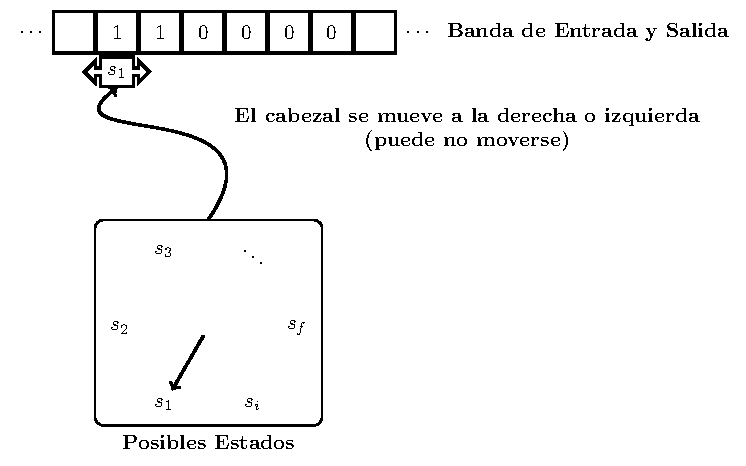
\includegraphics[scale=1]{images/fig_1.pdf}
            \end{center}
            \caption{Ejemplo de Máquina de Turing}
        \end{figure}
    \end{center}

   El cabezal $c$ puede moverse a la derecha, izquierda o no moverse, dependiendo del estado en el que esté. En la Figura \ref{Turing1} se muestra que el hay al menos 5 diferentes estados, desde el estado inicial ($s_i$) hasta el final ($s_f$). Dependiendo de la entrada, la función $T$ nos dirá lo que hará el cabezal, si cambia un elemento de la banda, si se mueve o si cambia de estado (o todas a la vez).

   En este ejemplo, el alfabeto sería $L=\left\{0,1 \right\}$, el conjunto de estados es $S=\left\{s_i,s_1,...,s_f \right\}$ y la función sería representada por lo que sea que haga el cabezal.

    \begin{exa}
        Considere $L=\left\{1 \right\}$, $S=\left\{s_i,s_1,s_2 \right\}$ y,
        \begin{equation*}
            T=\left\{(s_i,*,s_1,*,>),(s_i,1,s_1,1,>),(s_1,1,s_1,1,>),(s_1,1,s_2,1,-) \right\}
        \end{equation*}
        La cinta se ve más o menos así:

    \end{exa}

    Para los siguientes ejercicios, ir a la página: \href{https://turingmachinesimulator.com/}{Simulador Máquina de Turing}.

    \begin{excer}
        Codifique una máquina de Turing que sume 1 a un número dado en binario.
    \end{excer}

    \begin{lstlisting}
        name: Sumar uno en unario
        init: s0
        accept: sf

        
        // Funciones de Transicion

        s0,_
        s0,_,>

        s0,1
        s1,1,-

        s0,0
        s1,0,-

        s1,1
        s1,0,>

        s1,0
        s1,1,>

        s1,_
        sf,_,-

        // < = left
        // > = right
        // - = hold
        // use _ for blank cells

        // States and symbols are case-sensitive

        // Load your code and click COMPILE.
        //  or load an example (top-right).
    \end{lstlisting}

    \begin{excer}
        Codifique una máquina de Turing que dada un número en binario, invierta su orientación, es decir, si la cadena es $(a_1,...,a_n)$, que la máquina de Turing la convierta en $(a_n,...,a_1)$. 
    \end{excer}

    \begin{lstlisting}
        name: invertirCadena
        init: s0
        accept: s1,sf,l,c,u
        
        //esto para que se empiece a mover
        s0,_
        s0,_,>
        
        s0,0
        x,0,<
        
        s0,1
        x,1,<
        
        x,_
        s1,2,>
        
        s1,0
        s1,0,>
        
        s1,1
        s1,1,>
        
        //logica cuando encuentre cosas
        
        s1,_
        s2,_,<
        
        s2,_
        s2,_,<
        
        s2,0
        c00,_,>
        
        s2,1
        u00,_,>
        
        //mueve cosas al inicio
        
        c00,_
        m,0,<
        
        u00,_
        m,1,<
        
        //ya en ciclo
        
        //mueve derecha
        
        m,_
        l,_,<
        
        l,_
        l,_,<
        
        l,0
        c0,_,>
        
        l,1
        u0,_,>
        
        c0,_
        c0,_,>
        
        //mueve izquierda
        
        u0,_
        u0,_,>
        
        c0,0
        c1,0,>
        
        c0,1
        c1,1,>
        
        u0,0
        u1,0,>
        
        u0,1
        u1,1,>
        
        c1,0
        c1,0,>
        
        c1,1
        c1,1,>
        
        u1,0
        u1,0,>
        
        u1,1
        u1,1,>
        
        c1,_
        m,0,<
        
        u1,_
        m,1,<
        
        m,0
        m,0,<
        
        m,1
        m,1,<
        
        l,2
        sf,_,>
        
        sf,_
        sf,_,>
        
        sf,0
        sff,0,-
        
        sf,1
        sff,1,-        
    \end{lstlisting}


    \chapter{Teoremas de Completud}



\end{document}